\thispagestyle{fancy}
\fancyhead[R]{A.U 2025-2026}
\fancyhead[L]{Chapitre 3 : Sprint 1 -- Socle de la plateforme}

\chapter{Sprint 1 : Socle de la plateforme de supervision}

\section*{Introduction}
Ce chapitre est dédié à la première phase d'implémentation de la plateforme,
correspondant au \textbf{Sprint 1} du projet. Il constitue le socle fonctionnel du
système sur lequel s'appuieront tous les sprints suivants.

Ce sprint couvre l'authentification sécurisée des administrateurs, la mise en place de
l'agent Python de collecte, l'enregistrement automatique des serveurs supervisés ainsi
que la visualisation des métriques système en temps réel à travers un tableau de bord.

L'objectif de ce sprint est de disposer, à son issue, d'une chaîne complète et
fonctionnelle allant de la collecte d'une métrique sur un serveur jusqu'à son affichage
en temps réel dans l'interface, l'ensemble étant protégé par une authentification.

\section{Backlog du Sprint 1}
Après la définition des objectifs du Sprint 1, les \textit{User Stories} sélectionnées
à partir du \textit{Product Backlog} ont été décomposées en tâches techniques afin de
faciliter leur implémentation et leur suivi. Le tableau~\ref{tab:backlog-sprint1}
présente le backlog détaillé du Sprint 1.

\renewcommand{\arraystretch}{1.4}
\begin{longtable}{|>{\raggedright\arraybackslash}p{4.1cm}
                  |>{\raggedright\arraybackslash}p{7.7cm}
                  |>{\centering\arraybackslash}p{2.4cm}|}
\hline
\textbf{User Story} & \textbf{Tâches} & \textbf{Estimation} \\
\hline
\endfirsthead

\hline
\textbf{User Story} & \textbf{Tâches} & \textbf{Estimation} \\
\hline
\endhead

\hline
\multicolumn{3}{r}{\textit{Suite du tableau à la page suivante}} \\
\endfoot

\hline
\caption{Backlog du Sprint 1}
\label{tab:backlog-sprint1}
\endlastfoot

En tant qu'administrateur, je veux me connecter à la plateforme.
& Développer l'API d'authentification (\texttt{POST /api/auth/login}). & 1 \\
& Implémenter le hachage des mots de passe avec bcrypt. & 1 \\
& Générer et signer le jeton JWT (validité 24 h). & 1 \\
& Développer le middleware \texttt{verifyToken} de protection des routes. & 1 \\
& Réaliser l'interface de connexion React. & 1 \\
& Tester la fonctionnalité. & 1 \\
\hline

En tant qu'administrateur, je veux rester connecté et me déconnecter.
& Développer l'API de validation du jeton (\texttt{GET /api/auth/me}). & 1 \\
& Persister le jeton côté client (\texttt{localStorage}). & 1 \\
& Implémenter la déconnexion sécurisée. & 1 \\
& Tester la fonctionnalité. & 1 \\
\hline

En tant qu'agent, je veux collecter les métriques système toutes les 5 secondes.
& Développer le module de collecte Python avec \texttt{psutil}. & 2 \\
& Implémenter la lecture du CPU, de la RAM, du disque et du réseau. & 1 \\
& Développer le module d'envoi HTTP avec session persistante. & 1 \\
& Implémenter la logique de reprise en cas d'échec réseau. & 2 \\
& Externaliser la configuration (\texttt{config.json}, variables d'environnement). & 1 \\
& Tester la collecte et l'envoi. & 1 \\
\hline

En tant que système, je veux recevoir et persister les métriques.
& Concevoir les modèles Mongoose \texttt{Server} et \texttt{Metric}. & 1 \\
& Développer l'endpoint de réception \texttt{POST /metrics}. & 2 \\
& Implémenter l'enregistrement automatique d'un nouveau serveur. & 1 \\
& Développer le service de calcul de statut (\texttt{StatusService}). & 2 \\
& Indexer la collection des métriques pour optimiser les requêtes. & 1 \\
& Tester la persistance. & 1 \\
\hline

En tant qu'administrateur, je veux consulter le tableau de bord des serveurs.
& Développer l'API de liste des serveurs (\texttt{GET /api/servers}). & 1 \\
& Développer l'API de synthèse globale (\texttt{GET /api/dashboard/summary}). & 1 \\
& Réaliser l'interface du tableau de bord React. & 2 \\
& Implémenter l'affichage du statut par code couleur. & 1 \\
& Tester la fonctionnalité. & 1 \\
\hline

En tant qu'administrateur, je veux visualiser les métriques en temps réel.
& Mettre en place le canal WebSocket côté serveur. & 2 \\
& Développer la diffusion des mises à jour (\texttt{broadcastUpdate}). & 1 \\
& Implémenter le client WebSocket côté React. & 1 \\
& Développer le rafraîchissement automatique de l'interface. & 1 \\
& Tester la diffusion temps réel. & 1 \\
\hline

En tant qu'administrateur, je veux consulter l'historique des métriques.
& Développer l'API d'historique (\texttt{GET /api/servers/:id/metrics}). & 1 \\
& Implémenter le filtrage par période et par limite. & 1 \\
& Réaliser les graphiques de visualisation. & 2 \\
& Tester la fonctionnalité. & 1 \\
\hline

\end{longtable}

\section{Diagramme de cas d'utilisation du Sprint 1}
Dans cette section, nous présentons le diagramme de cas d'utilisation correspondant aux
fonctionnalités développées lors du premier sprint, tel qu'illustré dans la
figure~\ref{fig:uc-sprint1}.

\begin{figure}[H]
\centering
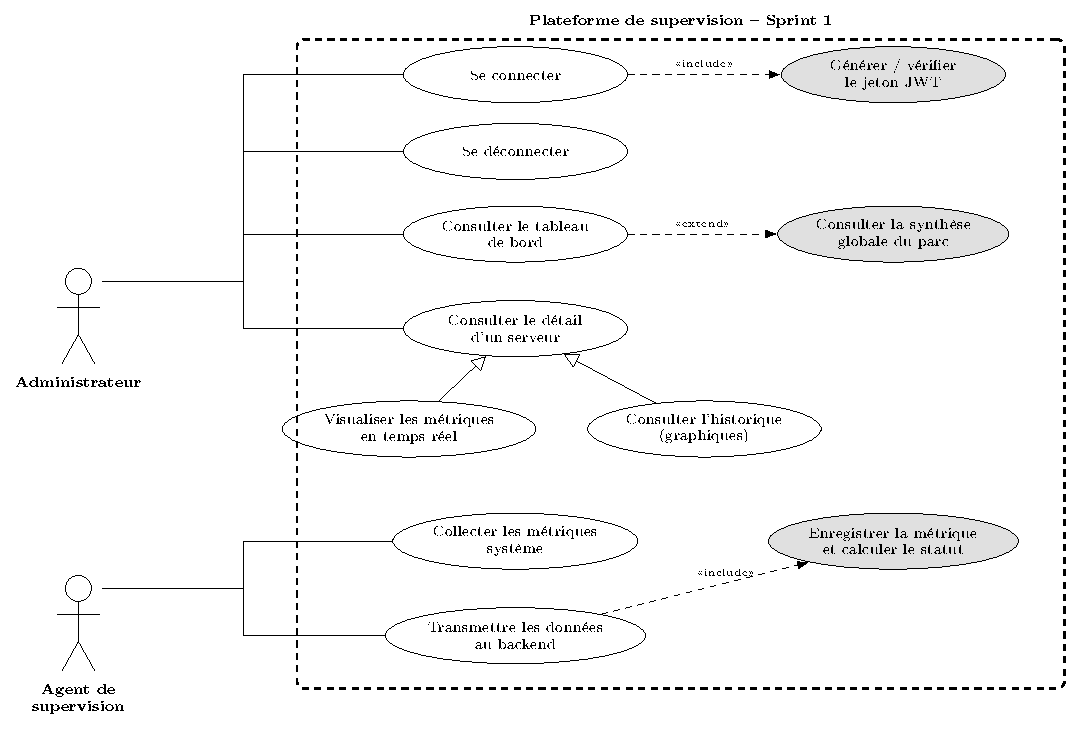
\includegraphics[width=0.92\textwidth]{figures/uc-sprint1.pdf}
\caption{Diagramme de cas d'utilisation du Sprint 1}
\label{fig:uc-sprint1}
\end{figure}

\section{Services Web du Sprint 1}
Les services Web constituent une interface permettant à deux applications de
communiquer via le réseau. Dans cette section, nous présentons la liste des services web
composant l'API de notre plateforme pour le Sprint 1. Ces services sont résumés dans le
tableau~\ref{tab:ws-sprint1}.

\renewcommand{\arraystretch}{1.3}
\small
\begin{longtable}{|p{1.6cm}|p{7.0cm}|p{5.8cm}|}
\hline
\textbf{Méthode} & \textbf{URL} & \textbf{Description} \\
\hline
\endfirsthead

\hline
\textbf{Méthode} & \textbf{URL} & \textbf{Description} \\
\hline
\endhead

\hline
\multicolumn{3}{r}{\textit{Suite du tableau à la page suivante}} \\
\endfoot

\hline
\caption{Liste des services web du Sprint 1}
\label{tab:ws-sprint1}
\endlastfoot

\multicolumn{3}{|c|}{\textbf{Authentification}} \\
\hline
\texttt{POST} & \texttt{/api/auth/login} & Se connecter avec email et mot de passe, et obtenir un jeton JWT. \\
\hline
\texttt{GET} & \texttt{/api/auth/me} & Valider le jeton stocké et récupérer le profil de l'utilisateur connecté. \\
\hline

\multicolumn{3}{|c|}{\textbf{Collecte des métriques}} \\
\hline
\texttt{POST} & \texttt{/metrics} & Recevoir les métriques transmises par l'agent Python et déclencher le calcul de statut. \\
\hline

\multicolumn{3}{|c|}{\textbf{Gestion des serveurs}} \\
\hline
\texttt{GET} & \texttt{/api/servers} & Récupérer la liste de tous les serveurs supervisés avec leur statut courant. \\
\hline
\texttt{GET} & \texttt{/api/servers/:server\_id} & Consulter le détail d'un serveur et sa dernière métrique. \\
\hline
\texttt{GET} & \texttt{/api/servers/:server\_id/metrics} & Récupérer l'historique des métriques d'un serveur sur une période donnée. \\
\hline
\texttt{POST} & \texttt{/api/servers} & Enregistrer manuellement un nouveau serveur. \\
\hline
\texttt{PUT} & \texttt{/api/servers/:server\_id} & Modifier les informations d'un serveur. \\
\hline

\multicolumn{3}{|c|}{\textbf{Consultation des métriques}} \\
\hline
\texttt{GET} & \texttt{/api/metrics/latest} & Obtenir la dernière métrique de chaque serveur supervisé. \\
\hline
\texttt{GET} & \texttt{/api/metrics/history/:serverId} & Récupérer l'historique des métriques pour la construction des graphiques. \\
\hline
\texttt{GET} & \texttt{/api/metrics/stats} & Obtenir des statistiques agrégées (moyennes, minima, maxima). \\
\hline

\multicolumn{3}{|c|}{\textbf{Tableau de bord}} \\
\hline
\texttt{GET} & \texttt{/api/dashboard/summary} & Obtenir la synthèse globale du parc (santé, alertes, volume de métriques). \\
\hline

\end{longtable}
\normalsize

\section{Les cas d'utilisation du Sprint 1}

\subsection{Cas d'utilisation : « Se connecter »}
Dans cette partie, nous proposons une description textuelle accompagnée des diagrammes
de séquence système et objet relatifs au cas d'utilisation « Se connecter ».

\subsubsection*{Description textuelle}

\renewcommand{\arraystretch}{1.4}
\begin{longtable}{|p{3.0cm}|>{\raggedright\arraybackslash}p{11.4cm}|}
\hline
\textbf{Acteurs} & Administrateur \\
\hline
\textbf{Objectif} & Permettre à l'administrateur de s'authentifier sur la plateforme
de manière sécurisée et d'obtenir un jeton d'accès lui donnant droit aux fonctionnalités
protégées, depuis l'application web comme depuis l'application mobile. \\
\hline
\textbf{Pré-condition} & L'administrateur doit disposer d'un compte actif enregistré
dans la base de données, avec le rôle \texttt{admin}. \\
\hline
\textbf{Scénario principal} &
\begin{enumerate}[leftmargin=*, nosep]
  \item L'administrateur accède à la page de connexion et saisit son adresse email et
        son mot de passe.
  \item Le système vérifie que les deux champs sont renseignés.
  \item Le système recherche l'utilisateur correspondant à l'adresse email.
  \item Le système compare le mot de passe saisi avec l'empreinte stockée (bcrypt).
  \item Le système génère un jeton JWT signé contenant l'identifiant, l'email et le
        rôle de l'utilisateur, valable 24 heures.
  \item Le jeton est retourné au client, qui le persiste localement.
  \item L'administrateur est redirigé vers le tableau de bord.
\end{enumerate} \\
\hline
\textbf{Scénarios alternatifs} &
\textit{A1 : Champs manquants}
\begin{enumerate}[leftmargin=*, nosep]
  \item Le système renvoie une erreur 400 et le message « Email et mot de passe sont
        requis ».
\end{enumerate}
\textit{A2 : Utilisateur inexistant}
\begin{enumerate}[leftmargin=*, nosep]
  \item Le système renvoie une erreur 401 et le message « Cet email n'est pas
        enregistré ».
\end{enumerate}
\textit{A3 : Mot de passe incorrect}
\begin{enumerate}[leftmargin=*, nosep]
  \item Le système renvoie une erreur 401 et le message « Le mot de passe saisi est
        incorrect ».
\end{enumerate}
\textit{A4 : Base de données indisponible}
\begin{enumerate}[leftmargin=*, nosep]
  \item Le système renvoie une erreur 503 et informe l'utilisateur de l'indisponibilité
        temporaire du service.
\end{enumerate} \\
\hline
\caption{Cas d'utilisation : Se connecter}
\label{tab:cu-login}
\end{longtable}

\subsubsection*{Diagramme de séquence système}
La figure~\ref{fig:seq-sys-login} illustre le diagramme de séquence système associé à ce
cas d'utilisation, mettant en évidence les interactions entre l'administrateur et le
système lors du processus d'authentification.

\begin{figure}[H]
\centering
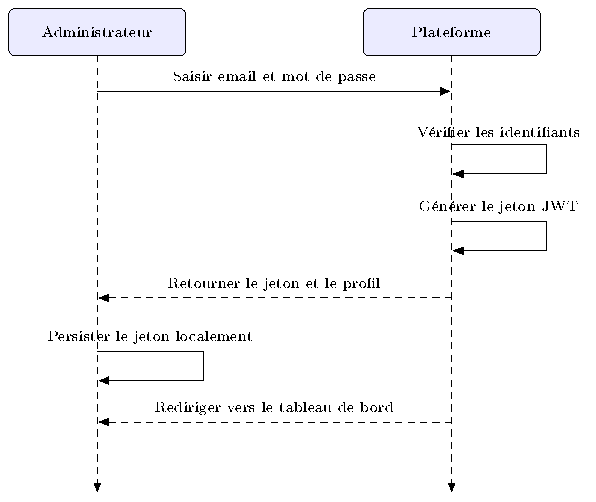
\includegraphics[width=0.9\textwidth]{figures/seq-sys-login.pdf}
\caption{Diagramme de séquence système du cas d'utilisation « Se connecter »}
\label{fig:seq-sys-login}
\end{figure}

\subsubsection*{Diagramme de séquence objet}
La figure~\ref{fig:seq-obj-login} illustre le diagramme de séquence objet associé au cas
d'utilisation « Se connecter », détaillant les interactions entre les composants internes
du système (interface, route d'authentification, modèle utilisateur et base de données).

\begin{figure}[H]
\centering
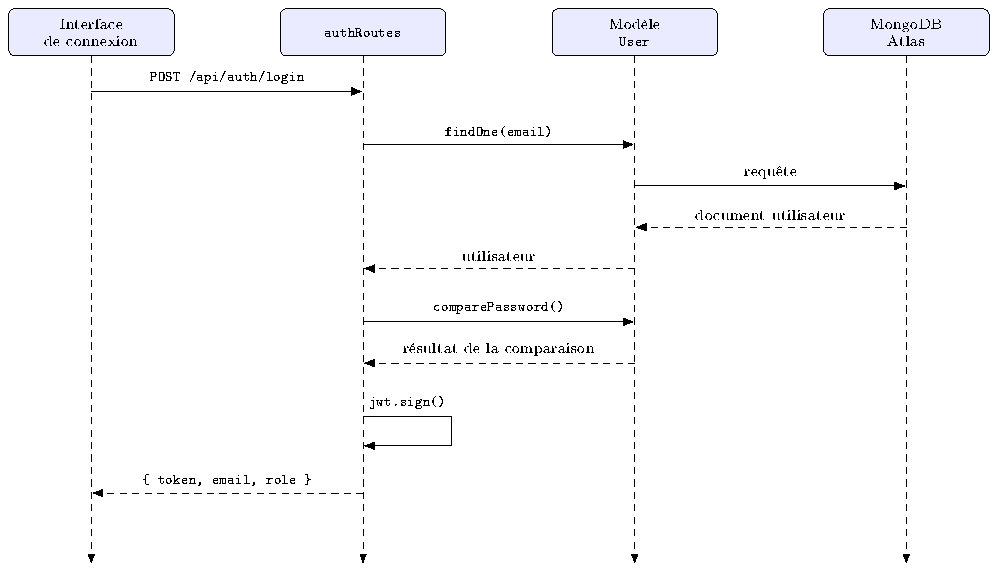
\includegraphics[width=\textwidth]{figures/seq-obj-login.pdf}
\caption{Diagramme de séquence objet du cas d'utilisation « Se connecter »}
\label{fig:seq-obj-login}
\end{figure}

\subsection{Cas d'utilisation : « Collecter et diffuser les métriques »}
Dans cette partie, nous présentons le cas d'utilisation central du Sprint 1, qui décrit
le cycle complet de la collecte d'une métrique jusqu'à son affichage en temps réel.

\subsubsection*{Description textuelle}

\renewcommand{\arraystretch}{1.4}
\begin{longtable}{|p{3.0cm}|>{\raggedright\arraybackslash}p{11.4cm}|}
\hline
\textbf{Acteurs} & Agent de supervision (déclencheur), Administrateur (destinataire) \\
\hline
\textbf{Objectif} & Collecter automatiquement les métriques système d'un serveur
supervisé, les transmettre au backend, calculer le statut du serveur et diffuser la
mise à jour en temps réel vers les clients connectés. \\
\hline
\textbf{Pré-condition} & L'agent Python est installé et configuré sur le serveur à
superviser. Le backend est accessible via le réseau. \\
\hline
\textbf{Scénario principal} &
\begin{enumerate}[leftmargin=*, nosep]
  \item L'agent collecte les métriques système à l'aide de \texttt{psutil} (CPU, RAM,
        disque, réseau, uptime).
  \item L'agent construit la charge utile en y ajoutant l'identifiant et le nom du
        serveur issus de sa configuration.
  \item L'agent transmet les données au backend via \texttt{POST /metrics}.
  \item Le backend vérifie la présence des champs obligatoires.
  \item Le backend recherche le serveur correspondant ; s'il n'existe pas, il est
        enregistré automatiquement.
  \item Le service de calcul de statut compare les valeurs reçues aux seuils configurés
        et détermine le statut (\texttt{OK}, \texttt{WARNING}, \texttt{CRITICAL}).
  \item La métrique est persistée et le document serveur mis à jour.
  \item Le backend diffuse la mise à jour à l'ensemble des clients connectés via
        WebSocket.
  \item L'interface met à jour l'affichage sans rechargement de page.
  \item L'agent attend 5 secondes puis recommence le cycle.
\end{enumerate} \\
\hline
\textbf{Scénarios alternatifs} &
\textit{A1 : Backend indisponible}
\begin{enumerate}[leftmargin=*, nosep]
  \item L'agent journalise l'échec et applique une temporisation exponentielle.
  \item Il poursuit ses cycles de collecte et reprend l'envoi dès le rétablissement de
        la connexion.
\end{enumerate}
\textit{A2 : Champs obligatoires manquants}
\begin{enumerate}[leftmargin=*, nosep]
  \item Le backend renvoie une erreur 400 et ignore la métrique reçue.
\end{enumerate} \\
\hline
\caption{Cas d'utilisation : Collecter et diffuser les métriques}
\label{tab:cu-collecte}
\end{longtable}

\subsubsection*{Diagramme de séquence objet}
La figure~\ref{fig:seq-obj-collecte} illustre les interactions entre l'agent Python et
les composants internes du backend lors d'un cycle de collecte.

\begin{figure}[H]
\centering
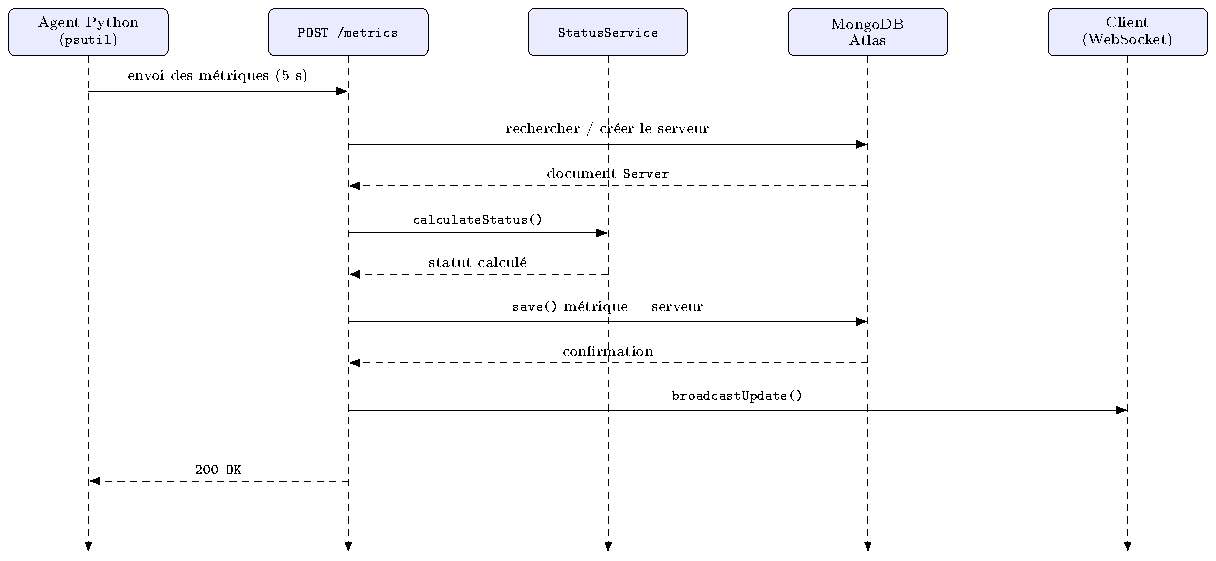
\includegraphics[width=\textwidth]{figures/seq-obj-collecte.pdf}
\caption{Diagramme de séquence objet du cas d'utilisation « Collecter et diffuser les métriques »}
\label{fig:seq-obj-collecte}
\end{figure}

\section{Réalisation du Sprint 1}

\begin{itemize}[label=\ding{220}]
\item \textbf{Interface de connexion :}
\end{itemize}
La figure~\ref{fig:real-login} illustre la page de connexion de la plateforme.
L'administrateur y renseigne son adresse email et son mot de passe. Une fois les
identifiants validés, un jeton JWT est généré et l'utilisateur est redirigé vers le
tableau de bord.

\begin{figure}[H]
    \centering
    \includegraphics[width=0.85\textwidth]{Image/real-login.png}
    \caption{Interface de connexion}
    \label{fig:real-login}
\end{figure}

\begin{itemize}[label=\ding{220}]
\item \textbf{Tableau de bord global :}
\end{itemize}
La figure~\ref{fig:real-dashboard} présente le tableau de bord principal. L'administrateur
y visualise l'ensemble des serveurs supervisés avec leur statut identifié par un code
couleur, les métriques courantes de chaque serveur ainsi qu'une synthèse globale de la
santé du parc.

\begin{figure}[H]
    \centering
    \includegraphics[width=0.9\textwidth]{Image/real-dashboard.png}
    \caption{Tableau de bord global des serveurs}
    \label{fig:real-dashboard}
\end{figure}

\begin{itemize}[label=\ding{220}]
\item \textbf{Détail d'un serveur et métriques en temps réel :}
\end{itemize}
La figure~\ref{fig:real-detail} illustre la page de détail d'un serveur. Elle affiche les
métriques instantanées (CPU, RAM, disque, réseau) mises à jour toutes les 5 secondes,
ainsi que les informations d'identification du serveur.

\begin{figure}[H]
    \centering
    \includegraphics[width=0.9\textwidth]{Image/real-detail-serveur.png}
    \caption{Détail d'un serveur et métriques en temps réel}
    \label{fig:real-detail}
\end{figure}

\begin{itemize}[label=\ding{220}]
\item \textbf{Historique des métriques :}
\end{itemize}
La figure~\ref{fig:real-graphiques} présente les graphiques d'historique permettant de
suivre l'évolution de la charge d'un serveur dans le temps et d'identifier
d'éventuelles tendances ou pics d'utilisation.

\begin{figure}[H]
    \centering
    \includegraphics[width=0.9\textwidth]{Image/real-graphiques.png}
    \caption{Historique des métriques sous forme de graphiques}
    \label{fig:real-graphiques}
\end{figure}

\begin{itemize}[label=\ding{220}]
\item \textbf{Exécution de l'agent Python :}
\end{itemize}
La figure~\ref{fig:real-agent} illustre la console d'exécution de l'agent de supervision
sur un serveur. Les journaux affichent chaque cycle de collecte et le résultat de la
transmission au backend.

\begin{figure}[H]
    \centering
    \includegraphics[width=0.85\textwidth]{Image/real-agent.png}
    \caption{Journaux d'exécution de l'agent Python}
    \label{fig:real-agent}
\end{figure}

\section*{Conclusion}
Ce chapitre a permis de présenter les fonctionnalités réalisées dans le cadre du
Sprint 1 de la plateforme. Ce sprint a permis la mise en place de l'authentification
sécurisée par jeton JWT, de l'agent Python de collecte des métriques système, de
l'enregistrement automatique des serveurs supervisés, du calcul de statut ainsi que du
tableau de bord temps réel alimenté par WebSocket.

Ces fonctionnalités constituent le socle technique de la plateforme et assurent une
supervision continue et fiable de l'infrastructure. Le chapitre suivant présente le
Sprint 2, consacré aux fonctionnalités d'administration : alertes, actions à distance,
sauvegardes et application mobile.
